\section{Systemarkitektur} \label{ch:Systemarkitektur}

Systemarkitekturen fungerer som udgangspunkt for designfasen af hele systemet.
Den danner overblik over det samlede systemet, hvorved det deles op i mindre blokke. 
De mindre blokke beskriver efterfølgende systemet i nærmere detaljer, således man kan derefter kan gå direkte til design af systemet. 

\begin{figure}[h]
\centering
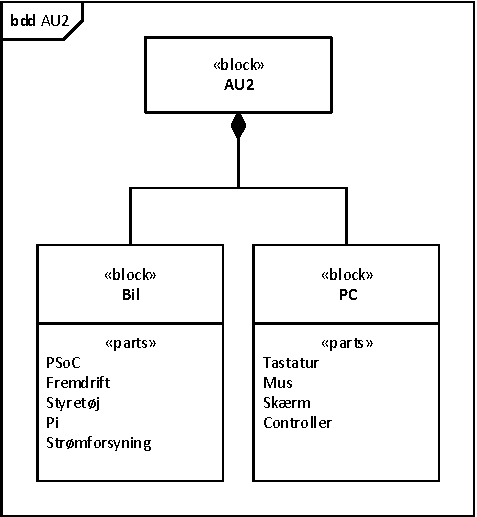
\includegraphics[width=0.5\textwidth]{../fig/diagrammer/bdd_au2.pdf}
\caption{Overordnet BDD for AU2}
\label{fig:bdd_au2}
\end{figure}

På figur \ref{fig:bdd_au2} ses et overordnet BDD for AU2. 
Det ses at systemet AU2 består af en bil og en PC. 
Bilen består af en \texttt{PSoC} som er et mikroprocessor-modul der styrer afstandssensorerne. 
\texttt{Fremdrift} er modulet der sikre bilens fremdrift, herunder motor osv. 
\texttt{Styretøj} er modulet der har med styretøjet at gøre, som gør det muligt for brugeren at dreje bilen. 
\texttt{Pi} er en Raspberry-Pi som er en computer der kører linux-styresystem, denne blok håndterer hele kommunikationen med PC'en. 
\texttt{Strømforsyning} er selve strømforsyningen til hele bilen, herunder: Motor, Pi, PSoC. 
\texttt{PC} af en Windows-computer med tilhørende tastatur, mus og skærm ,samt en Xbox-360 controller. 
På figur \ref{fig:bdd_bil} ses et udviddet BDD for bilen.  

\begin{figure}[H]
\centering
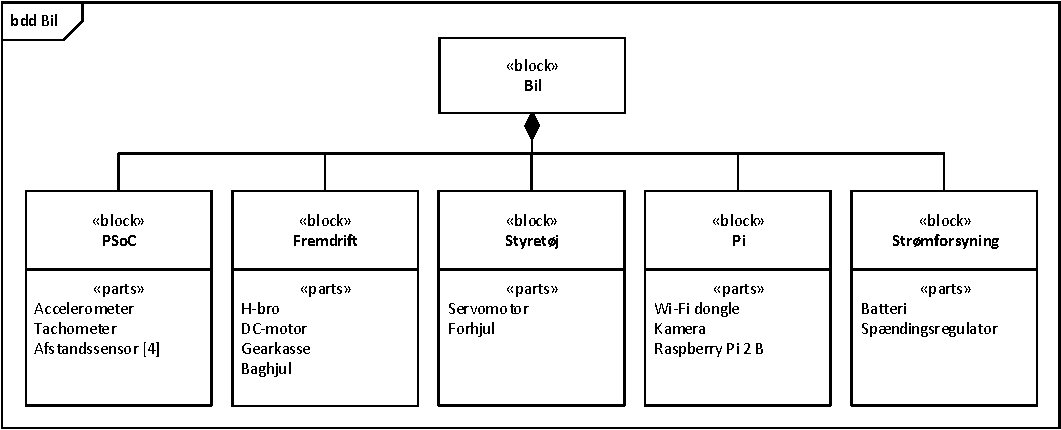
\includegraphics[width=0.7\textwidth]{../fig/diagrammer/bil/bdd_bil.pdf}
\caption{BDD for bil}
\label{fig:bdd_bil}
\end{figure}

På figur \ref{fig:bdd_bil} ses at \texttt{PSoC} består af et Accelerometer til at måle bilens acceleration, et tachometer til at måle bilens hastighed samt fire afstandssensor. 
\texttt{Fremdrift} består af en H-bro til at styre motorens omdrejningsvinkel, en DC-motor, en gearkasse og baghjul. 
Her er der dog to baghjul og ikke et som angivet i diagrammet. 
\texttt{Styretøj} består af en servomotor samt forhjul. 
\texttt{Pi} er bestående en  Raspberry-Pi som er påmonteret en Wifi-dongle samt et kamera. 
\texttt{Strømforsyningen} indeholder et batteri samt en spændingsregulator. Spændingsregulatoren er dog implementeret som en switchmode-powersupply.  

\begin{figure}[H]
\centering
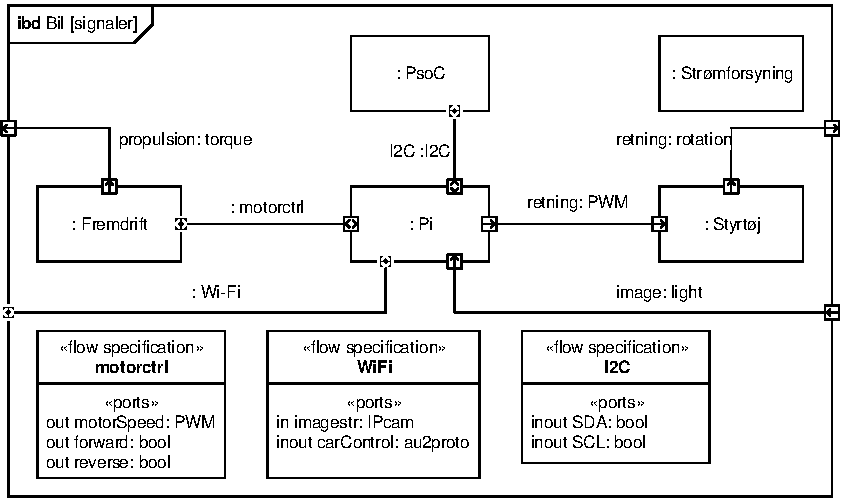
\includegraphics[width=0.7\textwidth]{../fig/diagrammer/bil/ibd_bil.pdf}
\caption{IBD for bil}
\label{fig:ibd_bil}
\end{figure} 

På figur \ref{fig:ibd_bil} ses ibd for bilen. 
Her er beskrevet hvilke signaler der forbinder blokkene samt deres indehold. 
Det ses at blokken \texttt{Fremdrift} er forbundet med motorctrl som er styringssignalet til motoren. 
Dette styrer motorens omdrejning og herved giver moment til hjulene. 
PcoC-modulet er kommunikerer med Pi'en via en \IIC forbindelse. 
Styretøjet styres med et PWM-signal hvor frekvensmodulationen er udtryk for hvor meget forhjulene drejer. 
Det ses også at Pi'en er koblet på et WiFi-netværk. 
I flow-specifications blokkene ses hvad signalerne indeholder af data. 
\texttt{motorctrl} indeholder, hastighed samt et signal om det er fremad eller bagud. 
WiFi indeholder kommunikationen med bilen samt et video-steam. \IIC indeholder blot \texttt{SDA} og \texttt{SCL} som er standart \IIC. 

\clearpage